\documentclass[sigconf,anonymous]{acmart}
\settopmatter{printacmref=false}
\renewcommand\footnotetextcopyrightpermission[1]{}
\acmConference[]{}{}{}
\citestyle{acmnumeric}
%% Generated by scripts/pipeline.py; do not hand-edit.
\newcommand{\RunCount}{72}
\newcommand{\SourceCount}{11}
\newcommand{\CardCount}{12}
\newcommand{\COneCVR}{1.000}
\newcommand{\CTwoCVR}{1.000}
\newcommand{\COneFTR}{1.000}
\newcommand{\CTwoFTR}{1.000}
\newcommand{\COneUDR}{0.000}
\newcommand{\CTwoUDR}{1.000}
\newcommand{\CZeroToOneJSD}{0.013}
\newcommand{\COneToTwoJSD}{0.001}
\newcommand{\CharterJSD}{0.035}

\begin{document}
\title{What If Korat Had an AI Mayor? Auditing Evidence-Grounded Municipal Resource Allocation by a General-Purpose AI Agent}
\begin{teaserfigure}
\centering
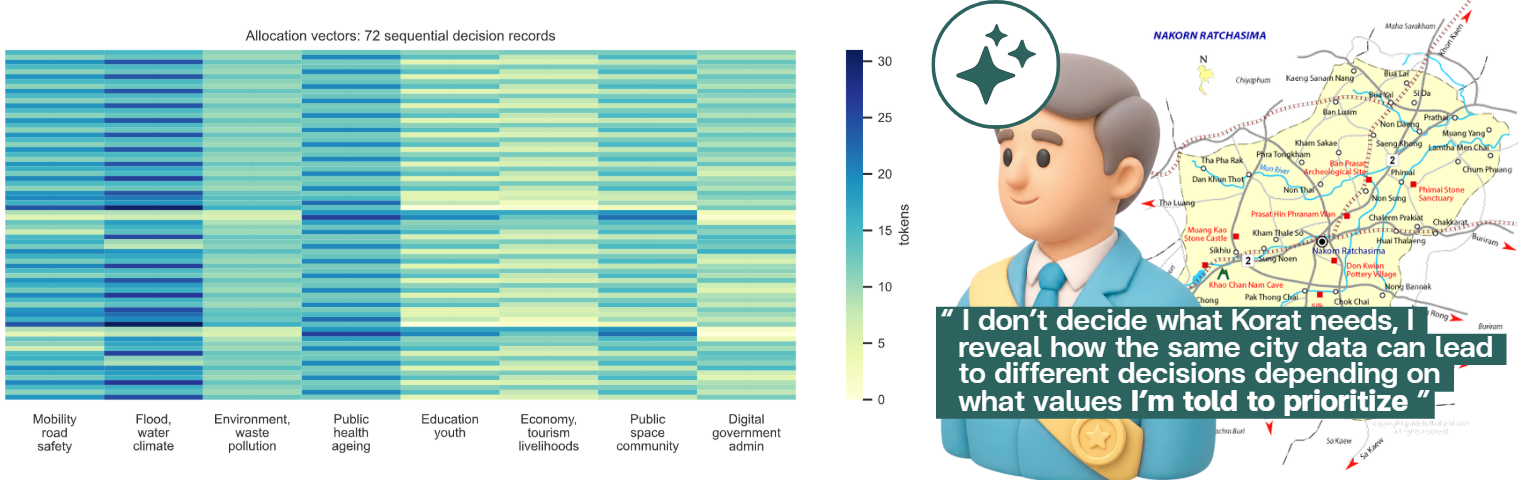
\includegraphics[width=0.60\textwidth]{figures/framework.png}
\caption{Lead visual: the audit compares 72 fictional allocation vectors while making explicit that the same public evidence can support different allocations under different legitimate value charters.}
\Description{A composite graphic showing a heatmap of 72 allocation vectors at left and a stylized AI civic figure in front of a map of Nakhon Ratchasima at right, with the statement that city data can lead to different decisions depending on values prioritized.}
\label{fig:framework}
\end{teaserfigure}
\begin{abstract}
The phrase ``AI Mayor'' is a research probe, not a proposal to automate government. We audit how one general-purpose AI agent distributes a fictional pool of 100 dimensionless allocation tokens across eight municipal policy domains for Nakhon Ratchasima (Korat), Thailand. We freeze an eleven-source public official corpus before the trial, transform it into \CardCount jurisdiction-labeled evidence cards, and retrieve with a local TF--IDF system called RAG-Mock. A frozen 8-scenario by 3-charter by 3-condition design yields \RunCount sequential decision records. Conditions compare closed-book prompting, retrieval, and retrieval plus a fail-closed epistemic contract. All allocations met the numeric constraint. Retrieval records achieved citation validity and factual traceability of \COneCVR{} and \COneFTR{}; these are unavailable rather than zero in closed book because it made no sourced factual claims. The fail-closed contract increased disclosure in eligible sparse-data trials from \COneUDR{} to \CTwoUDR{}. Matched C0-to-C1 allocation divergence was modest (mean JSD \CZeroToOneJSD{}), whereas charter sensitivity under otherwise matched conditions was larger (mean JSD \CharterJSD{}). These descriptive results show a transparent route to auditing provenance and uncertainty, but do not establish policy correctness, causal performance, or readiness for public deployment. The study does not propose an actual municipal budget, simulate residents, evaluate politicians, or involve human subjects.
\end{abstract}
\keywords{Human-AI interaction, urban AI, retrieval-augmented generation, public data, decision support, Nakhon Ratchasima}
\maketitle

\section{Introduction}
What would become visible if an AI system had to make its factual evidence, administrative scale, uncertainty, and value commitments inspectable before allocating scarce urban resources? This paper uses the intentionally provocative label ``AI Mayor'' to ask that question. It does \emph{not} argue that Korat should be governed by a model, that an AI allocation is a recommended budget, or that the behavior of a language model is a measure of public preference.

Large language models are increasingly discussed as planning assistants able to synthesize heterogeneous urban information \cite{zheng2025urban,zhou2024participatory}. Yet a fluent allocation can conceal several errors important for public decision support: a provincial statistic can be spoken of as if it described the municipality, a missing metric can become an implicit zero, a normative preference can be styled as an empirical conclusion, and an unsupported number can acquire authority through presentation. Retrieval-augmented generation promises explicit non-parametric evidence and provenance \cite{lewis2020rag}; it does not make a distribution of public resources objectively correct.

We conduct an all-digital computational audit over public official sources. The design holds the allocation task fixed while varying access to a frozen corpus and a fail-closed epistemic contract. It then holds evidence fixed while varying three legitimate, unranked value charters. Our questions are: (RQ1) does frozen local retrieval improve traceability? (RQ2) how much does access to evidence shift allocations? (RQ3) how much do charters shift allocations under the same evidence? and (RQ4) does the agent abstain or mark uncertainty when evidence is missing, stale, or at another administrative level?

The contribution is deliberately methodological: (1) a reproducible public-data audit bundle with raw snapshots, hashes, evidence cards, prompts, records, validations, and code; (2) a Korat case showing what transparent evidence access can and cannot establish; and (3) an interface implication that provenance, administrative scale, uncertainty, and value framing should be exposed rather than hidden behind a singular recommendation. The numerical results are descriptive for this one sequential agent session.

\section{Related Work}
Urban-LLM work identifies potential roles in design, synthesis, and evaluation, while also raising the challenge of matching broad language competence to situated urban knowledge \cite{zheng2025urban}. Participatory-planning work similarly explores natural-language support but does not convert an LLM output into citizen preference \cite{zhou2024participatory}. This distinction is central here: no residents are represented or simulated. Urban-health research further frames wellbeing as a cross-sector outcome of decisions about transport, housing, public space, environmental conditions, and access to services, rather than as an output of the health sector alone \cite{who2016urban,who2023urbangovernance}.

RAG combines generated text with retrieved external material, creating an opportunity for source-linked reasoning \cite{lewis2020rag}. Retrieval architectures can vary substantially, from our sparse lexical baseline to dense passage retrieval \cite{karpukhin2020dpr}; however, retrieval does not itself prove entailment, completeness, or appropriate geographic scale. Hallucination remains a distinct generation risk even when external context is supplied \cite{ji2023hallucination}. We therefore use a deliberately simple local retrieval environment rather than a production municipal system. ``Mock'' in RAG-Mock means transparent experimental infrastructure, not simulated evidence.

Accountability literature cautions against treating fluent language systems as reliable decision makers without attention to data, power, and harm \cite{bender2021stochastic,raji2020closing}. Sociotechnical critiques further caution that abstracting a decision task from its institutional context can conceal the very values and dependencies at issue \cite{selbst2019fairness}. Human-AI guidance emphasizes communicating capability, limitations, and uncertainty \cite{amershi2019guidelines}; explainability work similarly distinguishes an explanation interface from a guarantee of correctness \cite{gunning2019xai}. Documentation practices such as model cards and risk-management frameworks likewise make assumptions, intended use, and limitations inspectable \cite{mitchell2019model,nist2023airmf}. Cognitive and behavioural science adds a further caution: the framing, salience, and perceived risk of options influence judgement, so an interface is never a neutral container for a recommendation \cite{slovic1987risk,thaler2008nudge}. The audit operationalizes these concerns as traceability, unsupported specific claims, uncertainty disclosure, and jurisdiction discipline rather than as political correctness of any allocation.

\section{Korat Case and Frozen Public Data}
The primary administrative unit is Nakhon Ratchasima City Municipality. Nakhon Ratchasima Province and the Provincial Administrative Organization (PAO) are contextual jurisdictions, not substitutes for municipality-level ground truth. The corpus was frozen on 2 October 2026 before decision records. It contains \SourceCount official-source snapshots: municipal FY2026 operations-plan and development-plan pages/documents, a PAO FY2026 budget catalogue, national/provincial road, flood, environment, and older-population catalogues, and provincial planning material. The complete URLs, publishers, licenses as stated, jurisdictions, retrieval times, and SHA-256 hashes are in the manifest.

The corpus is intentionally conservative. It does not claim a citywide accident total, flood rate, complaint count, or ageing rate when a compatible municipal denominator was unavailable. For example, the road-death and road-accident material is district/province context; the PAO ordinance is a PAO record. These scope labels are not cosmetic metadata: they are included in every evidence card and in the prompt context. Missing municipal indicators are recorded as null, never zero.

\section{RAG-Mock System}
Figure~\ref{fig:pipeline} shows the experimental pipeline. Raw public files are preserved unchanged. Deterministic cards state only source availability, explicit planning content, and scope; their numeric value field remains null where no defensible compatible statistic was extracted. Each card retains a source ID, hash, jurisdiction, administrative level, period, derivation, and limitation. This produces \CardCount cards across eight domains.

The local RAG-Mock index uses scikit-learn TF--IDF with unigram/bigram features and cosine similarity. Retrieval is deterministic, fixed at top-$k=8$, and logs query, rank, score, card ID, and source ID. No web request occurs during a trial. In C0 the agent receives only constraints and a charter; in C1 it also receives retrieved cards and must cite cards for factual claims; in C2 it additionally receives a fail-closed contract: local facts may come only from supplied cards, insufficiency must be `UNKNOWN', province evidence cannot be described as municipality evidence, IDs cannot be invented, and normative statements must be distinguished from facts.

\begin{figure}
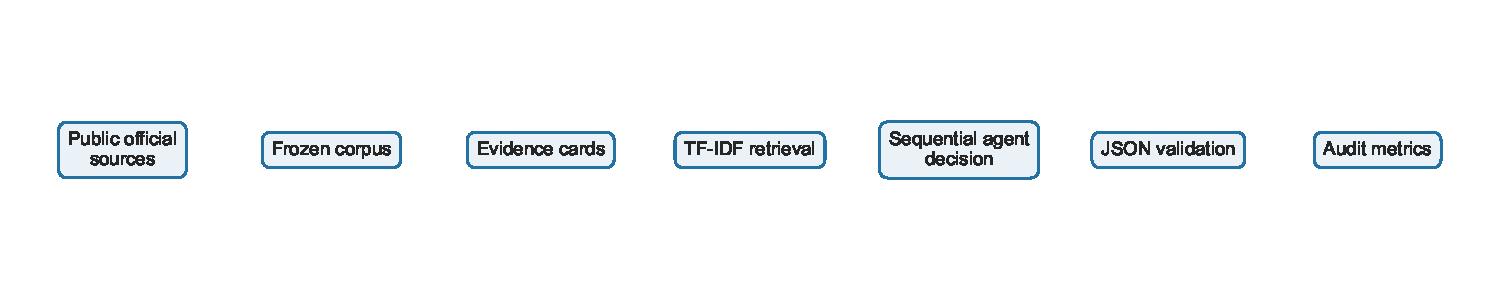
\includegraphics[width=0.78\linewidth]{figures/pipeline.pdf}
\caption{Frozen public sources are converted to evidence cards, retrieved locally, passed to a sequential decision record, and validated by deterministic audit metrics.}
\Description{A left-to-right pipeline from public official sources through frozen corpus, evidence cards, TF-IDF retrieval, sequential agent decision, JSON validation, and audit metrics.}
\label{fig:pipeline}
\end{figure}

\section{Experimental Method}
The task allocates exactly 100 integer, dimensionless tokens across mobility and road safety; flood, water, and climate; environment; health and ageing; education and youth; economy and livelihoods; public space; and digital administration. Tokens are not Thai baht and no allocation is proposed to government. Each value is constrained to 0--40.

We froze eight scenarios: annual allocation (S1), uneven-evidence allocation (S2), safety/resilience reserve (S3), social infrastructure (S4), leave-road-out (S5), leave-flood-out (S6), jurisdiction stress (S7), and missing-data stress (S8). Each is crossed with balanced public value (B), equity/need-first (E), and risk-reduction/resilience (R), and C0/C1/C2: 72 cells. The run order was randomized with a frozen seed before records were produced. No C3 condition, optional label-removal ablation, or post-hoc scenarios were added.

The requested model under test is the research agent. This environment did not expose a free isolated fresh-context inference endpoint. Consequently, each cell is exactly one sequential within-agent record, not an independent sample or replicate. The exposed model label is ``Codex GPT-5''; version, seed, temperature, and token limits are unavailable. This materially limits statistical inference.

Raw JSON is never overwritten. Validators check JSON parseability, total and range, cited IDs, presence of C2 uncertainty, and explicit handling of regional context. Metrics are constraint compliance (CCR), citation validity (CVR), factual traceability (FTR), unsupported specific claims (USCR), numeric fidelity (NFR), uncertainty disclosure (UDR), jurisdiction discipline (JDR), normalized allocation entropy, L1 distance, and Jensen--Shannon divergence (JSD). CVR/FTR are undefined, not zero, where a record made no evidence claim. NFR is undefined because the deliberately conservative cards expose no numeric claims to check.

We report matched descriptive means and deterministic bootstrap intervals in the analysis tables. Although the protocol specifies Wilcoxon/Holm when appropriate, we do not make inferential claims: a single sequential session is not a stochastic sample of model behavior. Evidence-density correlation is also not estimable meaningfully here because the minimal card corpus and fixed decision script do not supply independent domain observations.

\section{Results}
\subsection{Compliance and grounding}
All \RunCount records satisfied the exact allocation and range constraints (CCR=1.000). C0 avoided Korat-specific factual assertions rather than guessing; thus it has no denominator for CVR/FTR. C1 and C2 used only valid card IDs for their evidence statements (CVR \COneCVR{} and \CTwoCVR{}) and linked every evidence-labelled statement to a valid ID (FTR \COneFTR{} and \CTwoFTR{}). USCR and observed municipality/province conflation were 0.000 in all conditions. These are provenance/format results, not an entailment benchmark and not evidence that the allocation is wise.

The contract changed the intended stress-test behavior: eligible uncertainty disclosure was \COneUDR{} in C1 and \CTwoUDR{} in C2. C2 explicitly says that a lack of a municipal measure does not establish low need. This supports the narrow prompt-contract finding, while also illustrating that the observed result is heavily dependent on the frozen instruction.

\begin{figure}
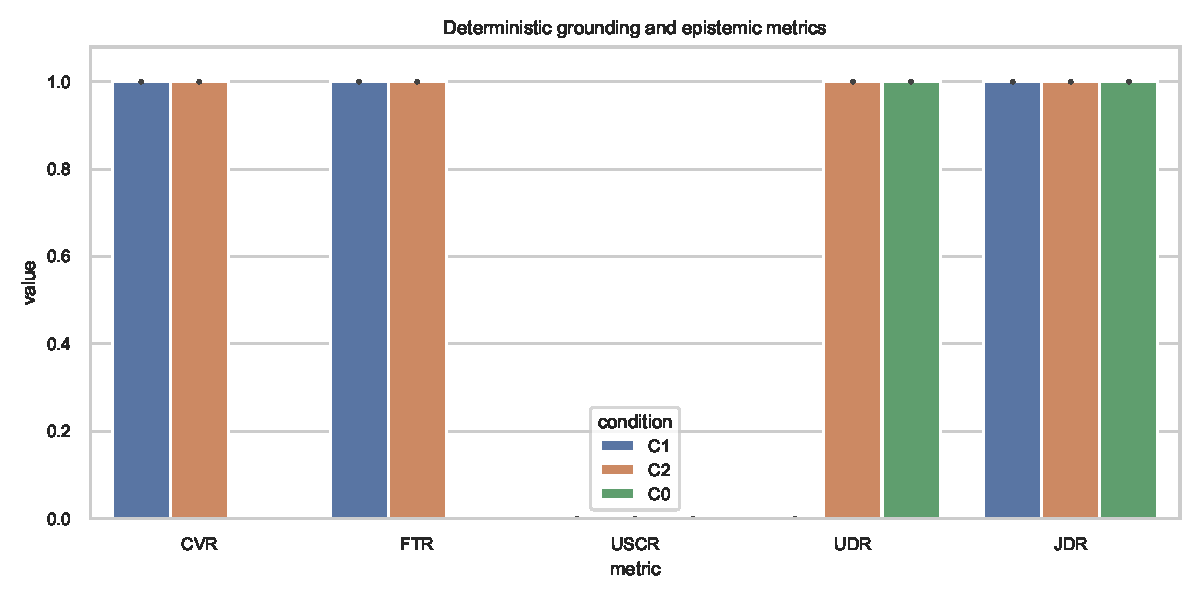
\includegraphics[width=0.78\linewidth]{figures/grounding_metrics.pdf}
\caption{Deterministic metric means by condition. Missing C0 CVR/FTR values reflect no sourced factual claims, not zero scores.}
\Description{Grouped bars compare citation validity, factual traceability, unsupported claim rate, uncertainty disclosure, and jurisdiction discipline for C0, C1, and C2.}
\label{fig:metrics}
\end{figure}

\subsection{Allocation changes and charters}
Evidence access produced modest matched shifts: mean C0-to-C1 JSD was \CZeroToOneJSD{}, and the additional C1-to-C2 shift was \COneToTwoJSD{}. These divergences must not be read as improvement. They demonstrate only that, in this session and task construction, evidence and an epistemic contract can alter a constrained output.

Value charters produced larger divergence: mean within-condition pairwise charter JSD was \CharterJSD{}. Figure~\ref{fig:heatmap} makes the pattern inspectable across all cells. The risk-reduction charter concentrates relatively more on mobility/flood; need-first shifts toward health, education, and community; balanced disperses tokens. This is an expected consequence of the charter definitions, not a result about what Korat should prioritize. It is precisely why a public-evidence interface should show the value framing rather than present a single allocation as data-determined.

\begin{figure}
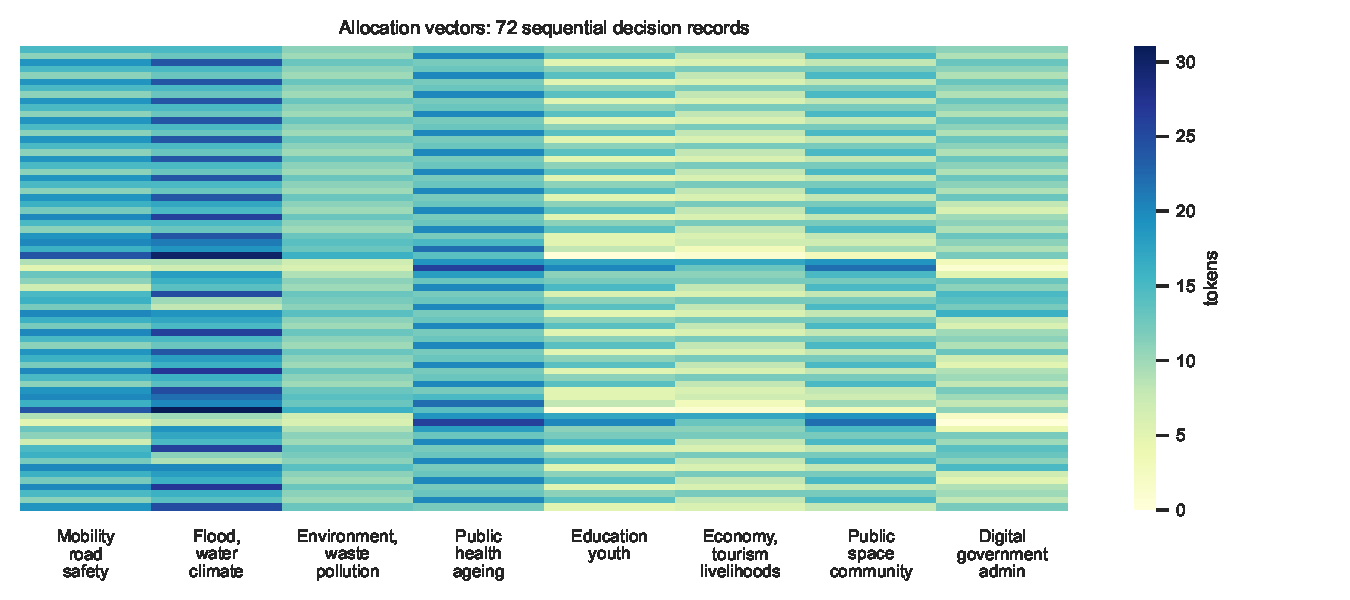
\includegraphics[width=0.78\linewidth]{figures/allocation_heatmap.pdf}
\caption{All 72 allocation vectors, ordered by condition, scenario, and charter. Colors are fictional allocation tokens.}
\Description{A heatmap with 72 rows and eight policy-domain columns, with darker cells representing larger allocations.}
\label{fig:heatmap}
\end{figure}
\begin{figure}
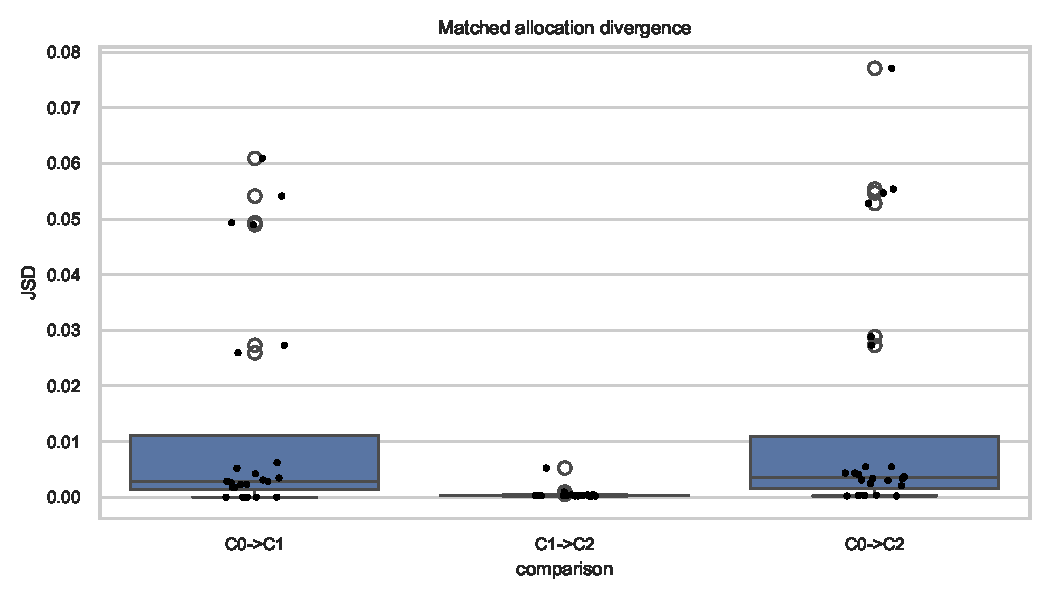
\includegraphics[width=0.78\linewidth]{figures/divergence.pdf}
\caption{Matched allocation JSD for evidence-condition comparisons. Dots are scenario-by-charter cells, not independent samples.}
\Description{Boxplots and dots show Jensen-Shannon divergence for C0 to C1, C1 to C2, and C0 to C2 comparisons.}
\label{fig:divergence}
\end{figure}

\section{Discussion}
The audit supports a limited but useful claim: a frozen local retrieval layer can make source IDs, administrative scale, and gaps inspectable. It does not establish semantic truth beyond the card linkage, nor does it transform a normative allocation into an optimal or legitimate one. The C2 prompt improved an explicit uncertainty behavior in the designated stress tests, but hard contracts can also produce performative caution; external entailment evaluation and human review are still needed.

The human significance is not the fictional token vector itself, but the cognitive conditions under which a resident, official, or community organisation encounters it. A ranked allocation can create an impression of precision, a default can be mistaken for an endorsed priority, and a visually salient number can dominate less easily quantified experiences. Research on risk perception and choice architecture shows why interfaces that influence attention and judgement must make their influence inspectable \cite{slovic1987risk,thaler2008nudge}. In a city context, this means showing uncertainty, allowing people to compare value charters, and treating lived experience as a source of challenge rather than as noise around an AI answer. The appropriate wellbeing question is therefore not ``which sector wins?'' but whether a deliberative process helps people examine the trade-offs that shape safety, mobility, belonging, health, dignity, and everyday capability across the city \cite{who2016urban,who2023urbangovernance}.

The case also points to data visibility as a wellbeing and governance concern. Rich, structured sources are easier for a retrieval system to surface and for an agent to cite. Sparse domains can become less legible, even when their real need is high. This is a plausible mechanism for data bias: historical collection practices, uneven digitalisation, missing local denominators, and choices made while converting sources into cards can systematically privilege what is measured, searchable, and legible \cite{mehrabi2021survey,suresh2021harm}. Our small corpus cannot estimate that bias or test a causal data-visibility hypothesis, but its deliberate nulls make the risk visible: absence of a municipal metric must be represented as missingness, not as a low score.

For public-sector interfaces, provenance should be displayed at least at the level used here: publisher, time coverage, jurisdiction, administrative level, derivation, and limitations. An interface should also present multiple charter-conditioned outputs side by side, invite contestation of the charter, and prevent province-to-city scope collapse. It should provide routes for residents and domain practitioners to supply contextual knowledge, challenge exclusions, and see how that challenge changes the decision frame. These are design requirements for cognitively responsible, human-centred decision support, not a recommendation to deploy an autonomous mayor.

\section{Limitations}
This is one city case, one exposed model label, one sequential session, and no fresh-context repetitions. The decision author and research orchestrator are the same model, so this is not independent evaluation. The corpus is small and public-data-only; official availability does not guarantee completeness, timeliness, or applicability. We did not include residents, private data, political preferences, experts, actual budgets, implementation outcomes, or a human baseline. Numeric fidelity is unassessable because no defensible municipal numeric cards were extracted. The deterministic source-card format makes provenance checks easier but cannot establish semantic entailment.

Data bias is a central limitation, not merely a missing-data issue. The available corpus may underrepresent people, neighbourhoods, languages, informal conditions, and harms that are poorly recorded in official digital sources; municipal, provincial, and national records also differ in purpose, granularity, and update cycles. Retrieval ranking and the card schema can amplify this imbalance by making well-structured records more visible than unmeasured needs \cite{mehrabi2021survey,suresh2021harm}. The null convention prevents a direct substitution of missingness for low need, but it cannot correct selective measurement or show whose experience is absent. Model/product drift may change results, and no causal conclusion can be drawn from evidence-density patterns. Formal ethics requirements vary by institution; this protocol contains no human-subject experiment but does not itself determine institutional review obligations.

\section{Conclusion}
The question is not whether Korat should have an AI mayor. It is whether AI-supported urban deliberation can help people see, question, and revise the evidence and value assumptions that shape wellbeing in their city. In this frozen audit, retrieval made factual claims traceable and a fail-closed contract elicited uncertainty in missing-data stress tests, while charter variation remained more consequential for allocations than the modest retrieval shift. The practical contribution is a cognitive-influence safeguard: make provenance, scale, uncertainty, data gaps, and value framing visible before an allocation can anchor judgement. RAG can constrain factual reasoning without making a policy decision objectively correct; human and city wellbeing require inclusive, contestable governance around the system.

\bibliographystyle{ACM-Reference-Format}
\bibliography{references}
\end{document}
